\section{Method}
\label{sec:method}
\method{} couples three decisions: what music to anticipate, how to express
the response as structured motion, and how to continue after committing it.
Figure~\ref{fig:overview} shows the complete system; the following figures
expand the reconstruction and continuation mechanisms.

\paragraph{Streaming task}
At decision time $\tau$, $a_{\leq\tau}$ is the heard audio, $h$ is committed
code history, and $b$ is the pose and velocity state reconstructed from the
last committed reference frames. A frozen music model predicts
$m^{\rm pred}=F(a_{\leq\tau})$, and the generator samples
\begin{equation}
(q_{1:H},r_{1:H})\sim p_\theta(q,r\mid h,b,m^{\rm pred}).
\label{eq:conditional}
\end{equation}
Here $q$ denotes discrete code indices and $r$ continuous residuals.
The codebook embeddings $e(q)$ are added to $r$ and decoded into
native G1 motion, conditioned on $b$. Both streams commit the same first $C<H$ steps; the
remaining plan is discarded. We use $H=8$ and $C=4$ at 15 latent steps per
second, yielding 16 planned and eight committed frames at 30\,Hz.

\subsection{Anticipatory Music Conditioning}
\label{sec:anticipation}
SpectroStream tokenizes heard audio, and frozen MRT-2 Small rolls forward to
predict musical states~\cite{magenta2026mrt2}. Its music pretraining supplies
the continuation prior; paired dance training learns how to turn that prior
into movement. Fourteen forecast states at 25\,Hz cover approximately
0.56\,s, alongside the 0.53\,s motion plan. Future waveform samples are never
used as input.

\paragraph{Align time before modulating features}
Forecast and motion steps have different rates, so matching array indices
would assign the wrong musical time. For state $u_j$ with physical lead
$\ell_j$ relative to the decision, we form
\begin{equation}
c_j=W\,\mathrm{LN}(u_j)+\phi(\ell_j).
\label{eq:music_projection}
\end{equation}
Here $W$ projects the music features and $\phi$ encodes their lead time.
We linearly interpolate neighboring projected states at motion lead
$d_i=i/15$ to obtain $\hat c_i$. A coverage mask
$m_i$ is one only within the valid forecast support and zero when the
condition is absent or no longer covers that motion time.

Each conditioned block adds a gated, frame-wise modulation
\cite{perez2018film}:
\begin{equation}
v'_i=v_i+m_i\,g\odot
\big[s(\hat c_i)\odot\mathrm{LN}(v_i)+t(\hat c_i)\big].
\label{eq:music_film}
\end{equation}
The learned maps $s,t$ predict scale and shift, and $g$ is a learned channel
gate. When $m_i=0$, the block retains its original activation exactly.
Separate modulators condition the structural Transformer blocks and residual
diffusion heads using the same physical-time alignment. The generator and
these mappings are trained; MRT-2 remains frozen.

\subsection{Structure--Detail Representation and Paired Training}
\label{sec:dc}
An encoder maps native motion and its starting state to $z=E_\varphi(x,b)$.
Quantization selects $q=Q(z)$ with codebook embedding $e(q)$, and a continuous
residual retains the remaining information:
\begin{equation}
z=e(q)+r.
\label{eq:latent}
\end{equation}
Both components are decoded by one boundary-conditioned decoder
$D_\psi(\cdot,b)$. Their roles are learned through complementary reconstruction
objectives, rather than separate anatomical decoders.

\paragraph{Learning complementary roles}
We train two reconstructions with the same decoder and starting state:
\begin{equation}
x_f=D_\psi(e(q)+r,b),\qquad x_s=D_\psi(e(q),b).
\label{eq:paired_paths}
\end{equation}
Both paths reconstruct complete motion through the same decoder.
The full-motion loss supervises all kinematic coordinates,
whereas the structure-only path uses only $e(q)$ as its motion
latent and is supervised on designated structural coordinates
(Fig.~\ref{fig:dc}).
For the full reconstruction, encoder gradients flow through $r$,
with $e(q)$ detached.
The structure-only reconstruction uses a straight-through estimator.
Both reconstruction losses update the shared decoder.
Codebook and commitment losses train the quantized representation;
Appendix~\ref{app:training} specifies the gradient routes.

The full loss supervises native coordinates, native velocities,
forward-kinematics positions, and geometry velocities. Each block is
standardized with training-set statistics and receives equal weight.
The structural loss uses the corresponding selected coordinates: root,
legs, and waist in the native views, and torso, wrists, and soles in the
geometry views. Consequently, wrist placement can be
structural while arm-joint articulation remains part of the complementary
native view. Auxiliary structural reconstruction under residual corruption
and a boundary-transition loss reinforce these objectives; their settings
and exact partitions remain in Appendix~\ref{app:training}.

\begin{figure*}[t]
\centering
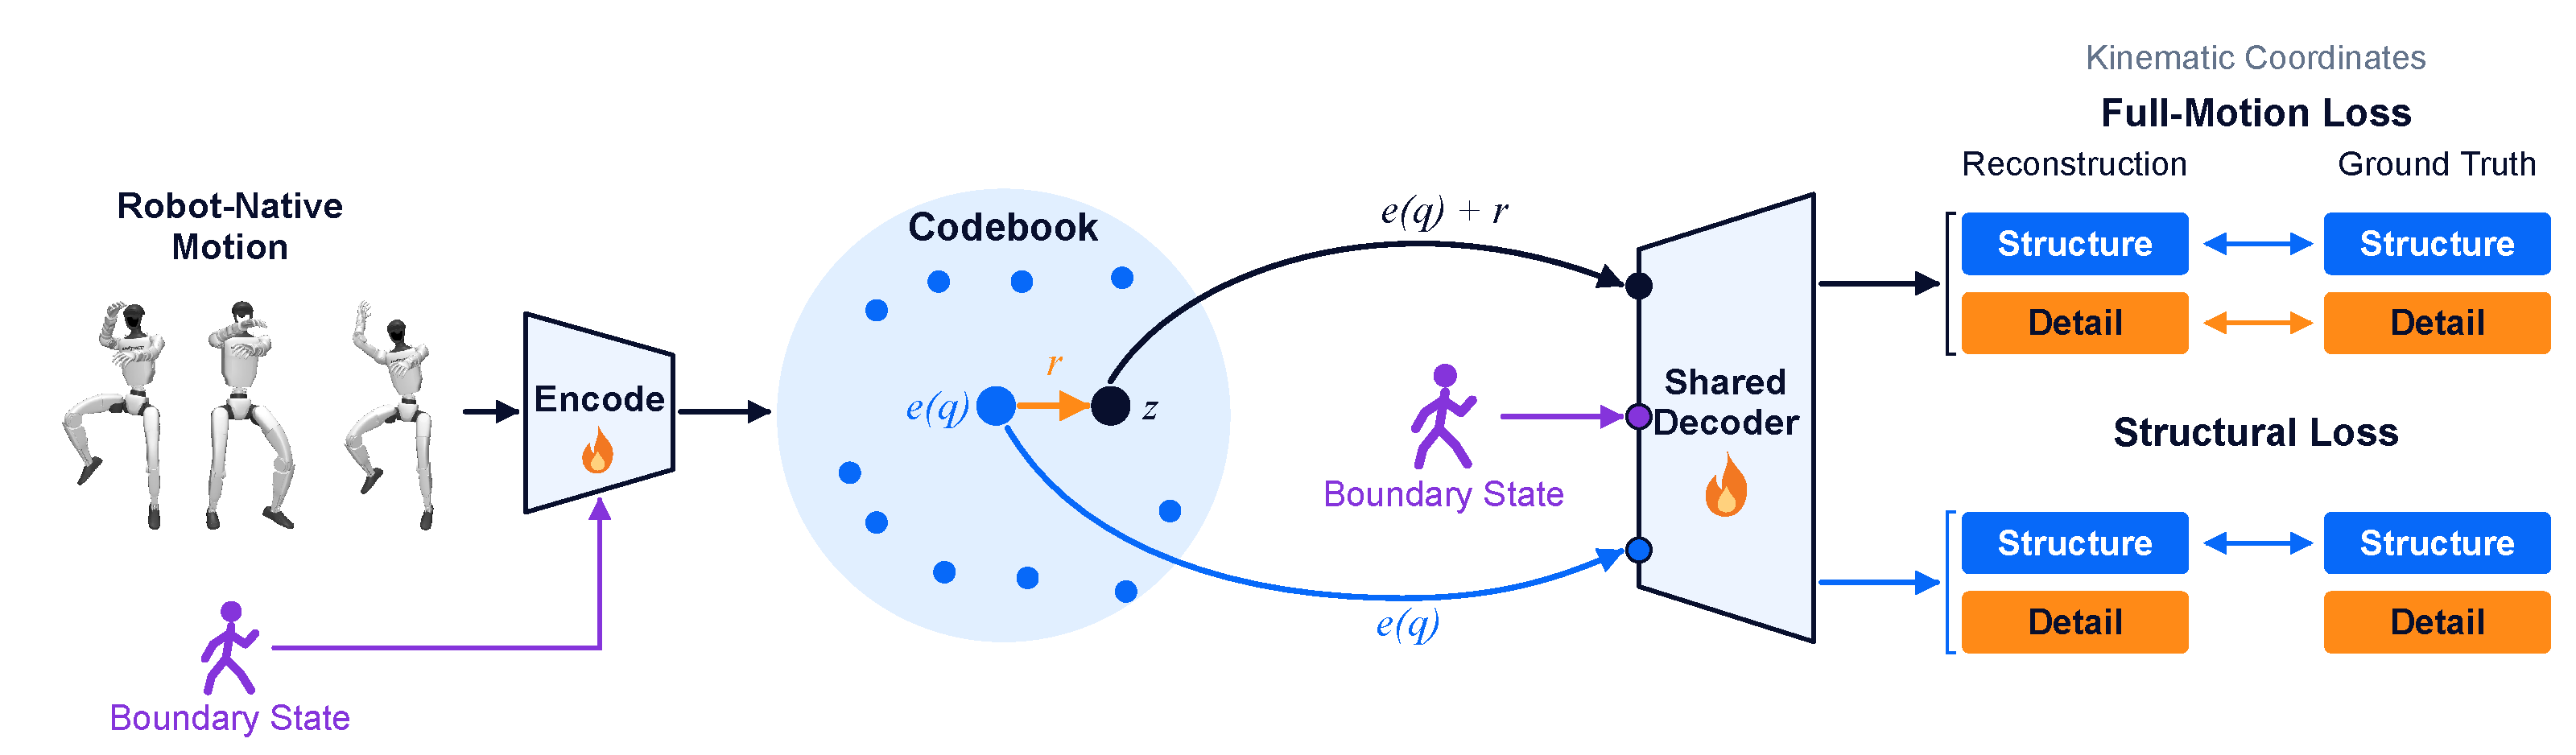
\includegraphics[width=\textwidth]{figures/foredance/structure-detail-training_refined_v3.pdf}
\caption{\textbf{Learning complementary structure and detail.} Core paired
reconstruction objectives. The encoder maps robot-native motion and its boundary
state to a latent composed of codebook embedding $e(q)$ and continuous residual $r$.
The shared decoder is evaluated twice with the same boundary state, using
$e(q)+r$ and $e(q)$. Both paths reconstruct complete motion. Blue and orange bands
denote structural and complementary kinematic coordinates, including velocities;
comparison links indicate which subsets enter each loss. Full-motion supervision
constrains both subsets, whereas structural supervision constrains only blue.
G1 poses, codebook geometry, and band widths are schematic; flames mark learned modules.}
\label{fig:dc}
\end{figure*}

\paragraph{Coupled motion generation}
A causal Transformer samples $q$. Its sampled IDs are embedded and added to
the residual model's input features; a diffusion generator
\cite{ho2020ddpm} samples $r$ using this structure, motion history, boundary
state, and aligned music. The codebook embedding and sampled residual then
sum at the shared decoder to produce 38-dimensional native motion. Joint
commitment preserves the pairing of the two streams across planning steps.

\subsection{Commit Forcing}
\label{sec:cof}
Teacher Forcing supplies ground-truth motion history and its boundary state;
streaming inference supplies both from the model's earlier output. Commit
Forcing changes this conditioning transition while retaining ground-truth
supervision for the subsequent motion (Fig.~\ref{fig:cof}).

\paragraph{Construct the next history and state together}
A first pass samples $\tilde q,\tilde r$ with the inference samplers under
stop-gradient. Their common committed prefix updates the two parts of the
next context:
\begin{equation}
(\tilde h^+,\tilde b^+)=U(h,b,\tilde q_{1:C},\tilde r_{1:C}).
\label{eq:joint_context}
\end{equation}
$U$ appends the committed codes to history and reconstructs the boundary
state from their decoded reference motion. Context replacement selects this
entire pair together, so generated history is accompanied by the state of
the same commitment. Each supplied training example constructs one such
transition independently; the first pass is not a recursive long rollout.

\paragraph{Keep the target, change its residual coordinates}
A second, gradient-enabled pass learns continuation conditioned
on the selected history--state pair.
The ground-truth motion for the next segment remains unchanged.
The ground-truth structural target $q^*$ and motion latent
$z^*=e(q^*)+r^*$ remain fixed.
The structure planner is supervised against $q^*$.
Its sampled code indices $\hat q$ are treated as constants
when conditioning residual denoising and constructing
the rebased residual target.
We express the residual target relative to that sampled embedding:
\begin{equation}
r^*_{\rm rebased}=z^*-e(\hat q),\qquad
e(\hat q)+r^*_{\rm rebased}=z^*.
\label{eq:rebase}
\end{equation}
Thus the structure and residual losses retain a common ground-truth target
latent despite a changed structural sample. This is latent rebasing, not
target re-encoding under $\tilde b^+$: the decoder also depends on its
boundary state, so latent equality does not imply identical decoded motion.

\begin{figure*}[t]
\centering
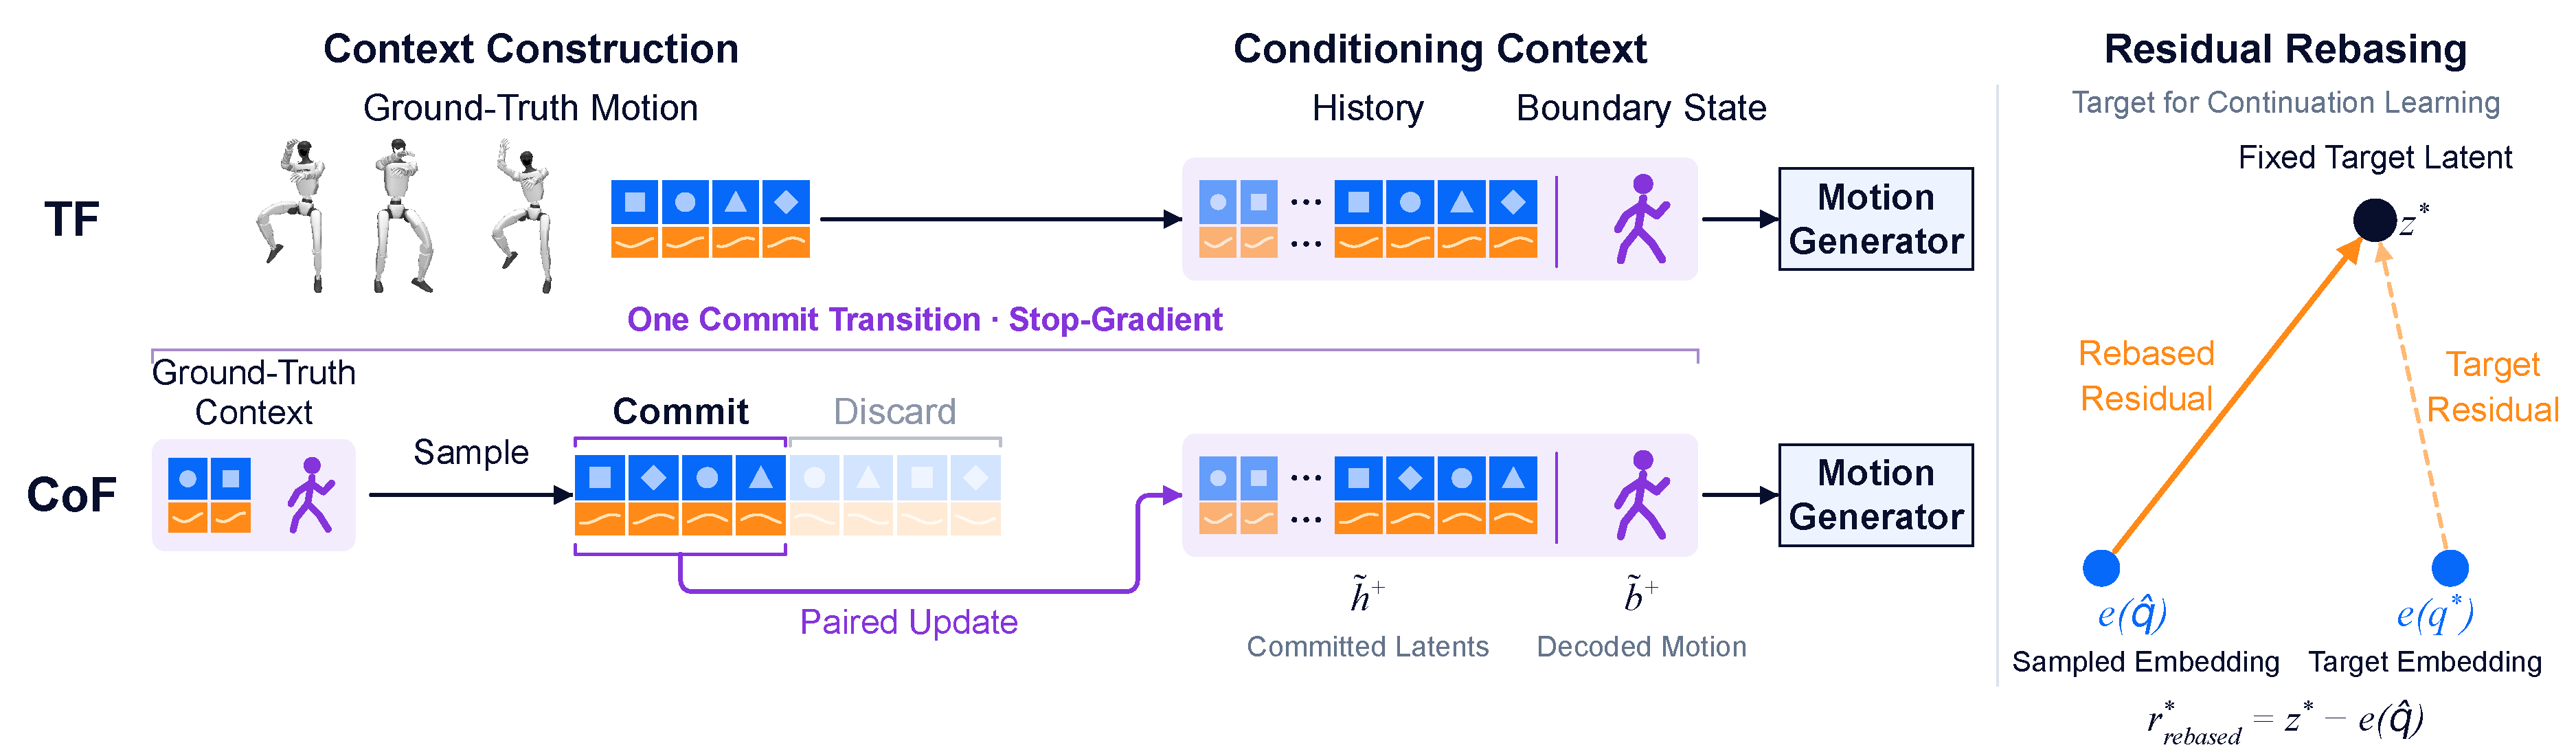
\includegraphics[width=\textwidth]{figures/foredance/cof-terminology_refined_v1.pdf}
\caption{\textbf{Constructing continuation contexts with Commit Forcing.}
TF uses ground-truth history and boundary state. CoF constructs one commit
transition under stop-gradient: committed latents update history, and decoded
motion determines the paired boundary state for continuation learning.
Residual rebasing keeps $z^*$ fixed and forms
$r^*_{\rm rebased}=z^*-e(\hat q)$ without re-encoding ground-truth motion at the
generated boundary. G1 poses, tile counts, and geometry are schematic.}
\label{fig:cof}
\label{fig:cof_training_detail}
\end{figure*}

\paragraph{History regularization}
After context construction, full-history corruption (FHC) perturbs discrete
embeddings and residuals across the motion history. It preserves boundary
state, music, masks, and timestamps, and is disabled during inference.
Appendix~\ref{app:training} specifies this separate training regularizer.

\subsection{Robot Reference Integration and Execution}
\label{sec:robot_execution}
Figure~\ref{fig:execution_interface} separates reference delivery from controller feedback. The committed native motion provides the reference interface to a separate, pretrained SONIC whole-body controller~\cite{luo2026sonic}. A reference bridge reconstructs root motion in the fixed sequence coordinate system, maps joint references into the controller convention, and resamples the 30\,Hz motion onto a continuous 50\,Hz grid. Appendix~\ref{app:training} defines the coordinates and state reconstruction. Only committed motion is delivered; the uncommitted suffix is discarded before the next plan and is not sent to the controller.

SONIC remains fixed and combines the consumed reference with measured robot state to produce control actions. The generator separately updates its latent history and boundary state from committed reference motion. Appendix~\ref{app:execution} specifies the delivery and measurement protocol.


% \begin{figure*}[t]
% \centering
% % Adapted from the execution path in teammate figures/architecture_v2.tex.
% Keep measured controller feedback separate from reference-only generation.
\resizebox{\textwidth}{!}{%
\begin{tikzpicture}[x=1cm,y=1cm,font=\sffamily\small,
 box/.style={draw=structure!75,fill=structure!4,rounded corners=2pt,align=center,text width=3cm,minimum height=1.25cm,inner sep=5pt},
 flow/.style={-{Latex[length=2.4mm]},thick,draw=structure},
 control/.style={flow,draw=detail},
 note/.style={font=\sffamily\footnotesize,align=center,fill=white,inner sep=3pt}]
\node[box] (ref) at (0,0) {Committed reference\\Native motion at 30\,Hz reference\\8 frames per commit};
\node[box] (bridge) at (4.3,0) {Reference bridge\\Root / joint conversion\\Continuous 50\,Hz grid};
\node[box,draw=detail!80,fill=detail!5] (sonic) at (8.6,0) {Fixed SONIC controller\\Reference tracking\\with measured state};
\node[box,draw=detail!80,fill=detail!5] (plant) at (12.9,0) {G1 in MuJoCo\\Executed motion};
\draw[flow] (ref) -- (bridge);
\draw[flow] (bridge) -- node[note,above,yshift=18pt,text width=1.6cm] {Delivered\\reference} (sonic);
\draw[control] (sonic) -- node[note,above] {Actions} (plant);
\draw[control] (plant.south) -- (12.9,-1.65) -- node[note,below] {Measured robot state} (8.6,-1.65) -- (sonic.south);
\node[box,text width=5.5cm,minimum height=.65cm] (context) at (1.8,1.9) {Generator history and boundary state};
\draw[flow] (ref.north) -- (context.south);
\node[note,anchor=west,text=structure] at (4.9,1.9) {Updated from committed references};
\node[note,anchor=west,text=detail] at (-1.6,-1.85) {Measured feedback remains inside the controller loop.};
\end{tikzpicture}%
}

% \caption{\textbf{From committed references to motion tracking.} The bridge converts the reference stream onto the controller grid. Committed references update the generator context, whereas measured robot state closes the SONIC tracking loop.}
% \label{fig:execution_interface}
% \end{figure*}

